\documentclass{article}
\usepackage{graphicx}
\usepackage{amssymb}
\usepackage{amsmath}
\usepackage{eurosym}
\usepackage{fullpage}
\usepackage{multirow}
\usepackage{fancyhdr}
\usepackage{amsmath}
\pagestyle{empty}
\usepackage{placeins}
\usepackage{changepage}
\usepackage[dvipsnames]{xcolor}
\usepackage{collectbox}
\usepackage{wrapfig}
\usepackage[utf8]{inputenc}
\usepackage[english]{babel}
\usepackage{gensymb}
\usepackage{tikz}
\usepackage{pgfplots}
\usepackage{graphicx}
\usepackage{booktabs}
\usepackage{enumitem}
\usepackage{afterpage}
\usepackage{overpic}
\usetikzlibrary{calc}
\usetikzlibrary{calc,patterns,angles,quotes}
\usepackage{xfrac}
\usetikzlibrary{automata, positioning}
\usepackage{color,soul}


\pgfplotsset{width=9cm,height=6.5cm,compat=1.9}

\setcounter{page}{1}


% Alternate method of doing solution function.
%\newcommand{\sol}[1]{}
%\renewcommand{\sol}[1]{{\color{blue} #1 \fi}}

%----------------------------------COMMANDS----------------------------------------------------
%---Create function to control text solution display----------------%
\newif\ifPrintSolution
\newcommand{\showSolution}{\PrintSolutiontrue}
\newcommand{\sol}[1]{\ifPrintSolution {\color{blue} #1 } \fi}
%---END Solution Function-------------------------------------------%

%---Create function to control R-Code solution display--------------%
\newcommand{\solR}[1]{} 
%---END R-Code Solution Function------------------------------------%

%%%%%%%%%%% Turn ON/OFF text solutions with this command%%%%%%%%%%%
\showSolution % comment out to hide solutions 
%%%%%%%%%%% Turn ON/OFF R-code solutions with this command%%%%%%%%%
\renewcommand{\solR}[0]{} % Comment out to hide R-Code Solutions

%------------------------------------------------------------------------------------------------

% Use \sol for text solutions and \solR for code chunk solutions

\begin{document}

\noindent \textbf{MA206 Lesson 4 - Strength of Evidence}
\vspace{.1in}


\textbf{What is Statistical Significance?}\\


\sol{Statistical Significance indicates the strength of evidence that the observed result was unlikely to have occurred by random chance}
\vfill

\textbf{What is the 3S Strategy?}

\sol{Statistic, Simulate, Strength of Evidence}
\vfill


What is the difference between a \textbf{parameter} and a \textbf{statistic}?

\sol{A parameter is the long-run behavior of a random process and it is not observable. A statistic is the summary of observed results and is used to infer about the parameter.}

\vfill

\textbf{Define:}

\hspace{.1in} \textbf{$H_0$} :\\
\sol{ Null Hypothesis, the ``Random Chance" model for the long-run behavior of the parameter.}
\vfill

\hspace{.1in} \textbf{$H_a$} :\\
\sol{ Alternate Hypothesis, the ``Something More" model for the long-run behavior of the parameter.}
\vfill

\hspace{.1in} \textbf{$\pi$} :\\
\sol{ The proportion parameter, the long-run behavior of a random process. It is unobservable.}
\vfill

\hspace{.1in} \textbf{$\hat{p}$} :\\
\sol{ The observed proportion statistic from data, used to argue or infer about the parameter}
\vfill

\hspace{.1in} \textbf{n} :\\
\sol{The sample size; The number of observations within each sample to construct the statistic}
\vfill

\hspace{.1in} \textbf{p-value} :\\
\sol{The probability of observing an observation at least as extreme as $\hat{p}$ assuming the null hypothesis is true.}
\vfill

Classify the strength of evidence for each range of p-values.

\begin{tabular}{ccccc}
\vspace{.1in}
0.1 & $< p$ & & & \sol{Weak Evidence against the null}\\
\vspace{.1in}
0.05 & $< p \le$& 0.1& & \sol{Moderate Evidence against the null}\\
\vspace{.1in}
0.01 & $< p \le$ & 0.05 & &  \sol{Strong Evidence against the null}\\
\vspace{.1in}
& $< p \le$ & 0.01 & & \sol{Very Strong Evidence against the null}
\end{tabular}


\pagebreak




\textbf{1) } MAJ McD's dreams of running West Point's best cookie bakery. To test his chances of success, he bakes chocolate chip cookies and has his cadets taste them in a blind comparison to two unnamed competitors. If we assume there is no difference in taste between the three cookies, we would expect an even distribution of preferences as cadet choice would be left to randomly guessing. This method was conducted among the class.

\hspace{0.2in}  For your class, what is the ratio of cadets that chose MAJ McD's cookie as their favorite?

\vfill

\hspace{0.2in} What is the ratio of cadets that chose mystery cookie K as their least favorite?

\vfill


\hspace{0.1in} \textbf{a) } What is the research question?

\sol{Do cadets prefer MAJ McD's cookies to the competitors, in general?}

\vspace{0.25in}

\hspace{0.1in} \colorbox{yellow}{\textbf{b) } What are the observational units in this study?}

\sol{The individual cadets in the classroom.}

\vspace{0.25in}

\hspace{0.1in} \textbf{c) } What are the variable(s)? Classify each as categorical or quantitative.

\sol{The variable is which cookie was chosen as the tastiest, and it is categorical (with three levels).}

\vspace{0.25in}

\hspace{0.1in}\colorbox{yellow}{ \textbf{d) } Describe the parameter of interest. What symbol is used to represent it?}

\sol{The parameter of interest is the proportion of people who choose MAJ McD's cookies over the competitors, represented by $\pi$}

\vspace{0.2in}

\hspace{0.1in} \colorbox{yellow}{\textbf{e) } For your class, list the appropriate values for the variables below and describe them in words.}

\vspace{0.1in} \hspace{0.2in}  \textit{n}: \sol{Will vary by class, generally 18;\\
The number of observations in the sample, aka the number of individuals given cookies and asked to choose one to eat. Here, class size.}

\vspace{0.1in} \hspace{0.2in} $\hat{p}$: \sol{Will vary based on class; The observed proportion of students in the class who choose MAJ McD's cookies as their favorite to eat. $\frac{Count \; who \; chose \; MAJ \; McD's}{Total \; cadets}$}

\vspace{0.1in} \hspace{0.2in} $H_0$: \sol{$\pi = \frac{1}{3}$. The null hypothesis. The true long run proportion of those who prefer MAJ McD's cookie is equal to  1/3  (the class will choose MAJ McD's cookie randomly.)}

\vspace{0.1in} \hspace{0.2in} $H_a$: \sol{$\pi > \frac{1}{3}$. The alternate hypothesis, the true long run proportion of cadets who will choose MAJ McD's cookie is greater than $\frac{1}{3}$}

\vspace{0.25in}

\hspace{0.1in} \textbf{f) } Is it possible for the sample to match the null hypothesis if the null hypothesis is false?

\sol{Yes, it is possible.}

\vspace{0.25in}

\hspace{0.1in} \textbf{g) } Is it possible to differ significantly from the null hypothesis if the null is true?

\sol{Yes, it is possible.}

\vspace{0.25in}

\hspace{0.1in} \textbf{h) } How might we use dice to randomly simulate and test our null hypothesis?

\sol{We might roll a 6-sided dice and select a 5 or 6 to represent a "success," or that someone chose MAJ McD's cookie. We could repeat this \textit{n} times for a sample of size \textit{n}, or alternatively roll \textit{n} dice and count the 5s and 6s.}

\vspace{0.25in}

\hspace{0.1in} \textbf{i) } Using the applets, run a simulation using your observed statistic, your hypotheses, and at least 1,000 simulations. Describe the null distribution. Describe where the observation falls (near the center or in the tails).

\sol{Answers may vary based on class output. There should be a sample size \textit{n} matching the class size, simulations of 1,000 or more, and probability of success of $\frac{1}{3}$. The distribution should be centered on 1/3, roughly normal looking, with variability from 0.08 to 0.67 (ish).}

\vspace{0.25in}

\hspace{0.1in} \colorbox{yellow}{\textbf{j) }  List your p-value from the simulation and describe the strength of evidence in words. Have we proven}\\ \colorbox{yellow}{the alternate hypothesis?}

\sol{Answers will vary. Strength of evidence should match the scale given in class. No, we have not proven the alternate hypothesis - it is still possible to get this result from chance, even if unlikely.

\vspace{0.2in}

\begin{tabular}{ccccc}
\vspace{.1in}
0.1 & $< p$ & & & \sol{Weak Evidence against the null}\\
\vspace{.1in}
0.05 & $< p \le$& 0.1& & \sol{Moderate Evidence against the null}\\
\vspace{.1in}
0.01 & $< p \le$ & 0.05 & &  \sol{Strong Evidence against the null}\\
\vspace{.1in}
& $< p \le$ & 0.01 & & \sol{Very Strong Evidence against the null}
\end{tabular}}

\vspace{0.2in}

\hspace{0.1in} \textbf{h) } Be able to repeat the above work for a different research question: Is the Keebler Chips Deluxe the least favorite cookie, in general? Repeat the analysis, provide a p-value, and write your conclusion.

\vspace{0.5in}

\textbf{2) } Many types of studies have been done to see whether animals have a sense of number. In one study (Beran $\&$ Beran, 2004), researchers wanted to see whether chimpanzees could remember how many items were added to a container when they see them added one at a time. To do this they had two containers set up so the chimpanzees could not see inside them. They randomly added bananas to the containers one at a time and then had the chimpanzees choose the container they wanted. In one set of experiments, they added 3 bananas to one container and 4 to the other and had a chimpanzee named Mercury pick which container he wanted. In 20 trials, he picked the container containing 4 bananas 16 times. 

\hspace{0.1in} \colorbox{yellow}{\textbf{a) } What is the observed statistic? Include the appropriate symbol.}

\sol{$\hat{p} = \frac{16}{20} = 0.8$}

\vspace{0.25in}

\hspace{0.1in} \colorbox{yellow}{\textbf{b) } In words and symbols, define the null and alternate hypotheses for this study.}

\sol{$H_0: \pi = 0.5.$ The long run proportion of times that Mercury picks the container with more bananas is 50$\%$.\\
$H_a: \pi \ge 0.5.$ The long run proportion of times that Mercury picks the container with more bananas is greater than 50$\%$.}

\vspace{0.25in}

\hspace{0.1in} \colorbox{yellow}{\textbf{c) } Below is a screenshot of a simulation done 100 times. What is the p-value, given our observed statistic} \colorbox{yellow}{and defined hypotheses? Comment on the strength of evidence.}

\begin{center}
    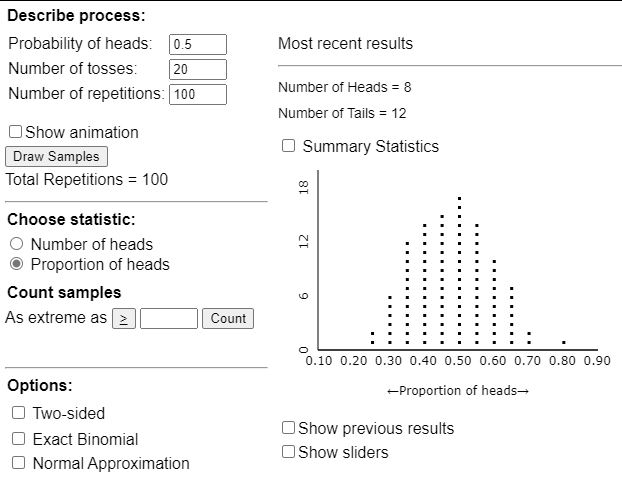
\includegraphics[scale=0.8]{2_Applet.JPG}
\end{center}

\sol{Our p-value is $\frac{1}{100} = 0.01$. This is very strong evidence against the null hypothesis that Mercury was choosing the boxes randomly.}

\vspace{0.25in}

\hspace{0.1in} \colorbox{yellow}{\textbf{d) } If we converted the null distribution to count of ``successes" instead of proportion, where would we}\\  \colorbox{yellow}{expect the above distribution to be centered on?}

\sol{We would expect it to be centered on 10. We have a $\pi$ = 0.5, \textit{n} = 20, and 0.5 $\times$ 20 = 10.}

\vspace{0.25in}

\hspace{0.1in} \textbf{e) } Given the above distribution, what is the fewest number of times that Mercury could pick the box with more bananas and we would still consider it strong evidence against randomly selecting boxes?

\sol{14 times. Above, a proportion 0f 0.70 has a p-value of 0.03, but a proportion of 0.65 has a p-value of 0.1. Strong evidence is $\le 0.05$, so we choose 0.70. With a sample size of 20, $0.7 \times 20$ = 14.}

\vspace{0.75in}

\textbf{3) } Your friend says he can shoot free throws as well as someone in the NBA and you don't think he is that good. You know that the NBA average for shooting free throws in the 2021-2022 season was 77.8$\%$. You test your friend by asking him to make 40 shots, and he makes 24 of them. Make a conclusion about your friend's claim, including your p-value.

\sol{$\hat{p} = \frac{24}{40} = 0.6$\\
$H_0: \pi = 0.778$\\
$H_a: \pi < 0.778$\\
p-value will change depending on simulation results, but should be about 0.008.\\
With a p-value of 0.008, we have very strong evidence against the null hypothesis that your friend is as good as an NBA player at making free throws.}


\end{document}
